%% This is free and unencumbered software released into the public domain.

%% Anyone is free to copy, modify, publish, use, compile, sell, or
%% distribute this software, either in source code form or as a compiled
%% binary, for any purpose, commercial or non-commercial, and by any
%% means.

%% In jurisdictions that recognize copyright laws, the author or authors
%% of this software dedicate any and all copyright interest in the
%% software to the public domain. We make this dedication for the benefit
%% of the public at large and to the detriment of our heirs and
%% successors. We intend this dedication to be an overt act of
%% relinquishment in perpetuity of all present and future rights to this
%% software under copyright law.

%% THE SOFTWARE IS PROVIDED "AS IS", WITHOUT WARRANTY OF ANY KIND,
%% EXPRESS OR IMPLIED, INCLUDING BUT NOT LIMITED TO THE WARRANTIES OF
%% MERCHANTABILITY, FITNESS FOR A PARTICULAR PURPOSE AND NONINFRINGEMENT.
%% IN NO EVENT SHALL THE AUTHORS BE LIABLE FOR ANY CLAIM, DAMAGES OR
%% OTHER LIABILITY, WHETHER IN AN ACTION OF CONTRACT, TORT OR OTHERWISE,
%% ARISING FROM, OUT OF OR IN CONNECTION WITH THE SOFTWARE OR THE USE OR
%% OTHER DEALINGS IN THE SOFTWARE.

%% For more information, please refer to <https://unlicense.org>
%%
\chapter{F-CSP}\label{fcsp}
This chapter describes F-CSP \cite{github:f-csp}, or Functional-CSP, a Scala
library with the intent of providing a functional constraint satisfaction
problem solver that can be easily integrated with Chisel. During the research
for this thesis, F-CSP was abandoned as a project, and section
\ref{sec:csp:whynotfcsp} explains why F-CSP was not developed further and how it
could have been improved.

\subsection{Introduction}
The idea behind F-CSP was to provide to the user a library that was seamless to
use inside a verification environment. Seamless in this context refers to a
natural language to use combined with Chisel. One of the benefits of using
verification languages with built-in constraint satisfaction utilities like
SystemVerilog is the natural interaction between classes and random objects.
This natural interaction is critical because it allows writing testbenches and
classes that are very expressive, without the need for code explanation or
comments. The second motivation was that, while there are relevant Java
libraries for solving constraint satisfaction problems see \cite{prudchoco4,
  online:jacop, online:optaplanner}, there are none for Scala, or at least there
are none published in Sonatype \cite{online:sonatype}. Third, Chisel is a
domain-specific language that leverages Scala's flexibility to provide the user
a DSL for hardware construction. Integrating a constraint satisfaction solver in
Chisel also means following the principles of Scala. Scala's flexibility allows
the user to write both functional and imperative programs, but it shines in the
former. These were the considerations that led to the creation of F-CSP. The
next section explains the requirements for creating a constraint programming
library for Chisel.

\section{Inspirations and requirements}
Like SystemVerilog is a combination of multiple languages unified by a standard,
and CoCoTb-coverage \cite{cieplucha2016new}, a library for code coverage and CRV
for CoCoTb, F-CSP was meant to be a library that would provide a constraint
programming on top of Chisel. When starting to prototype a new library or, in
this case, a domain-specific language about constraint, it is essential to
understand what are the requirements of the new language. Since the library will
be targeting a functional verification environment, the library must resemble
the language constructs familiar to verification engineers coming from a
different language. As shown in \cite{foster2015trends}, SystemVerilog is the
most commonly used language for verification and, as a countercheck,
CoCoTb-coverage was highly inspired by it. The last revision of SystemVerilog
language specification \cite{ieee2017ieee} shows that the language utilizes many
different keywords and general constructs to specify and solve random objects.
The keywords used are rand, randc, constraint, solve, before, soft, :=, :/, and
dist.

\begin{description}
    \item [rand] : rand is the keyword used to declare random fields inside a
      class. Any integer field inside a SystemVerilog object can be declared
      rand. Arrays can be declared rand. In this case, all its elements will be
      treated as random fields.
    \item [randc] : randc is the keyword used to declare random cyclic
      variables. randc variables permutate their value every time the object in
      which they are declared is randomized.
    \item [constraint] : constraint is the keyword that delimits the beginning
      of a constraint block. A constraint block is a list of expression
      statements that restrict a variable's range or defines relations between
      variables.
    \item [dist] : dist is the distribution operator, and it evaluates to true
      if the value of the expression is contained in the set; otherwise, it
      evaluates to false \cite{ieee2017ieee}. A weight to a set of values
      defined in a distribution can be assigned with the operators ``:=" and
      ``:/"
    \item[unique] : A group of variables can be constrained using the unique
      constraint so that no two group members have the same value after
      randomization.
    \item [if-else / ->]: The implication operator -> and if-else block are used
      to create conditional constraints based on a boolean predicate.
    \item [soft] : As the name says, soft constraints are constraints that have
      a lower priority compared to normal ones, and thus they are discarded when
      other more important ones contradict them.
    \item [solve, before] : The ``solve...before..." constraint specifies a
      partial ordering on the evaluation of variables. This partial ordering
      does not change the solution space.
\end{description}

Even if the number of keywords is relatively low, combining these keywords
creates complicated scenarios that can become quite hard to implement. Given the
author's hands-on inexperience with functional verification and how verification
engineers use the constraint language in SystemVerilog, it was decided to begin
with implementing only the most used keywords. Github was used to survey the
most used keywords in a verification environment, using its public searching
API. The search was conducted on the most popular SystemVerilog repositories,
which have more than 50 stars. The search resulted in 50 repositories in which
only 10 used random constraints for testing the design. Figure
\ref{fig:githubgraph} shows the results of the search. The results are not
representative and should not be used to reference how the verification engineer
works, but they give a starting point for the library development. From the
graph, it is clear that the most used keywords, other than \mints{rand} and
\mints{randc}, are \mints{dist} and \mints{solve...before..}. With these
parameters in mind, the work on the implementation was started.

\begin{figure}[ht]
\centering
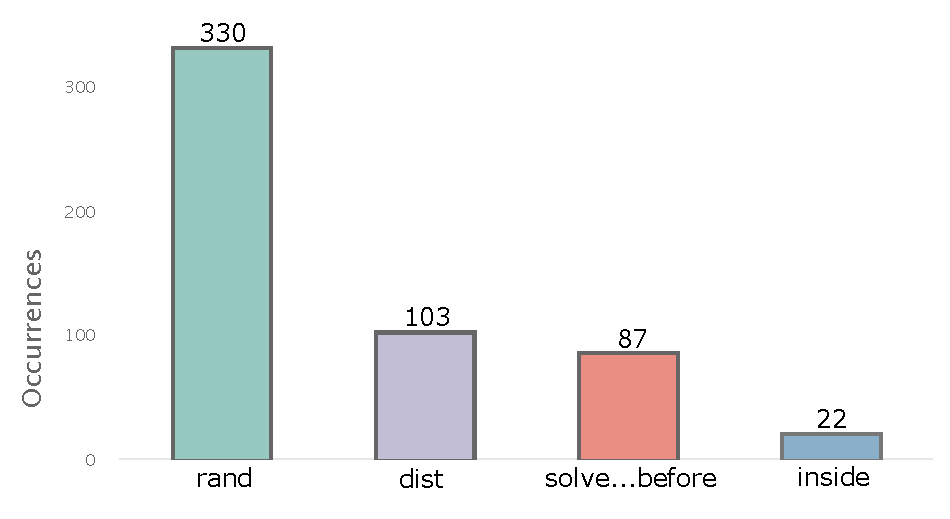
\includegraphics[width=0.7\linewidth]{pictures/Most_used_verification_keywords.eps}
\caption{Most used SystemVerilog's CRV keywords in Github.}
\label{fig:githubgraph}
\end{figure}

\section{Implementation}
As previously stated, the main goal with F-CSP was to create a pure functional
library able to solve constraint satisfaction problems, which could be easily
integrated with Chisel and provide a common language for expressing constraints.
The first step in implementing the library was to create a set of utilities and
classes to solve constraint satisfaction problems. As discussed in
\ref{sec:csp:def}, when solving constraint satisfaction problems for a hardware
description language, the domain types can be limited to discrete finite
domains. Secondly, without losing in generalization and as proven in
\cite{russell2002artificial}, it was decided to implement a CSP solver that only
accepted binary and unary constraints. As for other constraint satisfaction
problem solvers \cite{online:scala-csp, online:csp-solver-scala}, the main
algorithm inspirations were taken from the book \cite{russell2002artificial}.
The set of algorithms proposed was then modified to make it purely functional
\cite{github:f-csp}. The library contains six primary classes Variable, Domain,
CSP, Assignment, Solver, and Constraint. The next paragraph and sections
describe the API exposed and used in the library. Only the function's signatures
are reported for a matter of space, while the full implementation can be found
at \cite{github:f-csp}.

The library defines the concept of a CSP \mints{Variable} as a case class that
has only one field, the \mints{Variable}'s name. In a CSP, a \mints{Variable}
represents an entity that links a domain, a set of constraints, and a value.
Thus, Scala's case class constructor was a perfect choice for this entity since
it enables pattern matching. The \mints{Domain} class is also a Scala case class
that holds a \mints{List} of Scala \mints{BigInt} representing the
\mints{Variable}'s possible value. In this case, the case class was chosen for
convenience rather than its intrinsic properties. To represent a Domain, the
\mints{List} type was used instead of a \mints{Range} type, or the \mints{Array}
type since it was the only choice for properly handling noncontinuous domains
without introducing unnecessary copies of the domain values given that each
change of the domain leads to creating a new Domain class in order to maintain
the library's functional aspect. The \mints{Constraint} class is represented as
an interface using the Scala \mints{trait} constructor, which is realized by two
classes, \mints{Unary} and \mints{Binary} constraints. The interface exposes the
necessary methods for verifying that the current constraint is consistent with
the current CSP definition.


\begin{code}
\begin{minted}
[
frame=lines,
framesep=2mm,
baselinestretch=1.2,
fontsize=\footnotesize,
linenos
]
{scala}
trait Constraint {
  def isConsistent(variables: List[Variable], assignments: Assignments): Boolean
  def relatesTo(variables: List[Variable]): Boolean
  def isSatisfied(mapVariableValue: Map[Variable, BigInt]): Boolean
  def relatesToVar(variable: Variable): Boolean
  def getOther(variable: Variable): Option[Variable]
  def neighbor: List[Variable]
  def isUnary: Boolean
}
\end{minted}
\caption{\mints{Constraint} trait in F-CSP.}
\label{listing:constrainttrait}
\end{code}

By having defined the three main components of a CSP, \mints{Variable},
\mints{Domain}, and \mints{Constraint}, it is possible to proceed with the
definition of a Constraint Satisfaction Problem represented by the CSP case
class inside F-CSP. The CSP class represents the current state or ``definition"
of a problem to solve. The term ``current" relates to the fact that each time a
constraint is added or a value is assigned to a variable, the entire CSP class
is cloned by creating a new instance with the new parameters as shown by the
function signatures of \mints{removeUnary} and \mints{restrictDoamin} in listing
\ref{listing:cspclass}. Three parameters are used in this class: the list of
variables, a map linking variables and domains, and the list of constraints.
This case class exposes a few methods that are used to describe the
configuration of the current problem. Listing \ref{listing:cspclass} shows the
CSP class's methods. The term neighbors, in listing \ref{listing:cspclass},
refers to the variables linked to a specific variable with a constraint, as
shown in figure \ref{fig:crv:graph}; the term arcs refers to the edges or
constraint that link two variables.

\begin{code}
\begin{minted}
[
frame=lines,
framesep=2mm,
baselinestretch=1.2,
fontsize=\footnotesize,
linenos
]
{scala}
class CSP(val variables: List[Variable], val varDomMap: Map[Variable, Domain],
         val constraints: List[Constraint]) {
  def removeUnary(): CSP
  def restrictDomain(mapVarDomain: (Variable, Domain)): CSP
  def getConstraints(variables: List[Variable]): List[Constraint]
  def reviseArcs(Xi: Variable, Xj: Variable): List[(Variable, Variable)]
  def neighbors(variable: Variable): List[Variable]
  val combinationOfArcs: List[(Variable, Variable)]
}
\end{minted}
\caption{\mints{CSP} class in F-CSP.}
\label{listing:cspclass}
\end{code}

After defining the container that represents the current problem, it is possible
to proceed with the \mints{Assignment} definition. An \mints{Assignment} in
F-CSP represents a relation between a \mints{Variable} and a value. By
conforming with the library's functional nature, the \mints{Assignment} class is
also a case class that, every time a \mints{Variable} is assigned a value,
returns a new instance of the same class. The \mints{Assignment} class is just a
layer on top of a map between \mints{Variable} and value, by itself does not
know anything about the definition of the current CSP. Listing
\ref{listing:assclass} shows the main methods of the \mints{Assignment} class.

\begin{code}
\begin{minted}
[
frame=lines,
framesep=2mm,
baselinestretch=1.2,
fontsize=\footnotesize,
linenos
]
{scala}
case class Assignments(mapVarValue: Map[Variable, BigInt]
= Map[Variable, BigInt]()) {
  def apply(variable: Variable): BigInt
  def addValue(unassignedVar: Variable, value: BigInt): Assignments
  def getUnassignedVariable(variables: List[Variable], seed: Int = 42): Variable
  def assigned(variable: Variable): Boolean
  def areAssigned(variables: List[Variable]): Boolean
  def isComplete(variableList: List[Variable]): Boolean
  def isPartial(variableList: List[Variable]): Boolean 
}
\end{minted}
\caption{\mints{Assignment} class in F-CSP.}
\label{listing:assclass}
\end{code}

The last class is the \mints{Solution} class, which is extended from the trait
\mints{Node}. A node in this context refers to a node in the search graph.
Listing \ref{listing:nodeclass} shows the primary methods that the trait
\mints{Node} exposes. The same listing shows that the functions' signature is
different from the one presented in the book \cite{russell2002artificial}. The
first notable difference is that the AC-3 function returns an
\mints{Option[CSP]}. Returning an \mints{Option[CSP]} is necessary because the
AC-3 algorithm can return a refined \mints{CSP} or the \mints{None} type if the
CSP is not solvable. A second difference is the \mints{tailrec} notation applied
to the AC-3 implementation function. Using pattern matching in combination with
\mints{Option}, it is possible to move the recursive call of the AC-3 algorithm
as the final action of the procedure, and thus the compiler can optimize the
call stack and reduce the number of stack frames. The second difference is the
backtracking algorithm.

\begin{code}
\begin{minted}
[
frame=lines,
framesep=2mm,
baselinestretch=1.2,
fontsize=\footnotesize,
linenos
]
{scala}
trait Node[T] {
  def revise(csp: CSP, Xi: Variable, Xj: Variable): Option[Domain]
  def AC_3(csp: CSP, queue: List[(Variable, Variable)]): Option[CSP]
  @tailrec
  private def AC_3_imp(csp: CSP, queue: List[(Variable, Variable)]): Option[CSP]
  def isArcConsistent(csp: CSP): Boolean
  def MAC(csp: CSP, queue: List[(Variable, Variable)]): Option[CSP]
  def children(solution: T): Stream[T with Node[T]]
  def backtrackingSearch(csp: CSP): Stream[T with Node[T]]
  def backtrack(solution: T): Stream[T  with Node[T]]
  def selectUnassignedVar(solution: T): Variable
  def orderDomainValues(solution: T, variable: Variable): Stream[BigInt]
  def inference(solution: T, unassignedVar: Variable): Option[CSP]
}

case class Solution(csp: CSP, assignments: Assignments, seed: Int) 
extends Node[Solution] {
  def isConsistent(newAssignment: (Variable, BigInt)): Boolean 
  def isComplete: Boolean
  override def selectUnassignedVar(solution: Solution): Variable
  override def orderDomainValues(solution: Solution, variable: Variable): Stream[BigInt]
  override def inference(solution: Solution, unassignedVar: Variable): Option[CSP]
  override def MAC(csp: CSP, queue: List[(Variable, Variable)]): Option[CSP]
  override def children(solution: Solution): Stream[Solution with Node[Solution]]
  override def backtrackingSearch(csp: CSP): Stream[Solution with Node[Solution]]
  override def backtrack(solution: Solution = this): Stream[Solution with Node[Solution]]
}

\end{minted}
\caption{\mints{Node} and \mints{Solution} classes in F-CSP.}
\label{listing:nodeclass}
\end{code}


The return type of the backtracking method is a \mints{Stream} of lazily
computed \hfill \break \mints{Solutions}. This implies that each time the next
method is called on the \mints{Stream}, a new \mints{Solution} is computed on
demand. The backtracking search starts by removing all the unary constraints
defined in the CSP, thus reducing the domain of the variables defined in the
CSP. After that, following the functional paradigm, a new solution is created
with the new CSP and an empty assignment. Before starting the search, it is
possible to use the \mints{MAC} algorithm to refine the CSP. If the \mints{MAC}
algorithm returns a valid \mints{Solution}, the algorithm starts traversing the
solution tree until a possible solution is found.

\section{Constraint Language}\label{sec:csp:constraintlanguage}
After creating the set of primitives for solving constraint satisfaction
problems in Scala, it was necessary to create an interface between Chisel and
the library. To achieve the final goal of creating a seamless experience for the
user in writing constraints, F-CSP contains a package called crv. The crv
package is a collection of helper classes that allows the user to extend a
generic Scala class that can accept random fields and be randomized. Inside the
crv package, there are two main classes. The first one, called \mints{Random},
is what each random object should inherit from and exposes all the necessary
methods to create and declare random objects. The second one, called
\mints{RandomMacros}, contains all the declarations of the macros used in F-CSP.
The macros defined in this class are ``compile-time macros." The library uses
macros to detect which fields need to be randomized in the object. The Random
class uses the type \mints{RandInt} to declare a random field. This new type is
a refinement of the internal \mints{BigInt} type. This controversial choice,
which will be explained throughout the next paragraph and sections, had its
advantages and disadvantages. The main disadvantage was the impossibility to
detect at run-time which fields were declared random.

For this reason, compile-time macros were used to detect the field declared with
the \mints{RandInt} type, extract its name, create a variable with the same
name, and finally registered it inside a map linking random variable to its
domain in the \mints{Random} class. As an example, listing
\ref{listing:randexample} shows a declaration of a random field. In this case,
\mints{len}, the field has to be declared as a \mints{var} because it will be
updated during the object's randomization. The \mints{rand} macro accepts two
parameters, the field to be declared random and its domain. It is relevant to
note the potentials of Scala macros. In listing \ref{listing:randexample},
\mints{len} is a field that, during its declaration, is also used as an argument
to the \mints{rand} macro.

\begin{code}
\begin{minted}
[
frame=lines,
framesep=2mm,
baselinestretch=1.2,
fontsize=\footnotesize,
linenos
]
{scala}
 var len: RandInt = rand(len, 0 to 10 toList)
\end{minted}
\caption{\mints{Random} Field declaration in F-CSP}
\label{listing:randexample}
\end{code}

One of the significant benefits of having a refined type derived from a internal
type is the possibility of using it directly combined with other classes and
\mints{BigInt} variables. For example, it is possible to manipulate the value of
\mints{len} without any problem or compare it with other tests' values. This is
a clear advantage because it allows random fields in all the functions that
accept the BigInteger type without implicitly converting it.

\begin{code}
\begin{minted}
[
frame=lines,
framesep=2mm,
baselinestretch=1.2,
fontsize=\footnotesize,
linenos
]
{scala}
 len = 10
 assert(len < 100)
\end{minted}
\caption{Usage of random fields in F-CSP.}
\label{listing:usageoflen}
\end{code}

After the declaration of random fields, it is possible to add constraints to the
class. A constraint is declared by either using the Scala macro \mints{unary} or
\mints{binary}. The \mints{unary} macros accept one parameter, a lambda function
with the signature \mints{BigInt -> Bool}, while the \mints{binary} macro also
accepts as a parameter a lambda function but with the signature \mints{(BigInt,
  BigInt) -> Bool}. In this case, the macros are used to decompose the lambda
function at compile-time, detect the parameters name and the boolean function,
and create a constraint that links the parameters name with the corresponding
constraint. The return type of the constraints macros is a
\mints{ConstraintBlock} type. This type can contain one or more constraints, and
it adds two new methods, \mints{enable} and \mints{disable}, to conditionally
enable or disable the list of constraints inside the verification environment.

\begin{code}
\begin{minted}
[
frame=lines,
framesep=2mm,
baselinestretch=1.2,
fontsize=\footnotesize,
linenos
]
{scala}
val bConstraint = constraintBlock(
    unary (a => a >= 3),
    unary (a => a <= 4),
    binary ((a, b) => a + b = 10)
  )
  [...]
  ....multicast.disable()
\end{minted}
\caption{Constraint declarations in F-CSP.}
\label{listing:constdeclar}
\end{code}


Finally, the new random object can be instantiated and randomized with the
\hfill \break \mints{randomize} method. The \mints{randomize} method generates
the next value for all the random fields and return the result of the DFS inside
the CSP solver. \mints{randomize} is also a Scala macro because the
\mints{RandInt} type is just a refinement of the \mints{BigInt} type. For this
reason, \mints{randomize} is a compile-time macro that parses the abstract
syntax tree of the class to find all the declared random fields and assign the
new value them.

Listing \ref{listing:randobjscala}, shows an example of random a object declared
in F-CSP. Contrary to the SystemVerilog example in listing \ref{listing:3}, to
declare a random object, the user has to extend the class from the
\mints{Random} base-class provided by the library. After that, each random
variable has to be declared of type \mints{RandInt} and initialized with the
\mints{rand} macro. Finally, like for SystemVerilog, in Scala, inheriting the
\mints{Random} base class exposes the method \mints{randomize}, which assigns
random values to the class's random fields. The method \mints{randomize} returns
a \mints{Boolean} based on the result of the randomization.

\begin{code}
\begin{minted}
[
frame=lines,
framesep=2mm,
baselinestretch=1.2,
fontsize=\footnotesize,
linenos
]
{Scala}
class AluTransaction extends Random {
  var a: RandInt = rand (a, 0 to 255 toList)
  var b: RandInt = rand (b,  0 to 255 toList)
  var op: RandInt = rand (op, 0 to 7 toList)
  val valid = constraintBlock (
    binary { (a, b) => a + b < 255 },
    binary { (a, b) => a - b > 0 }
  )
}
[...]
val transaction = new AluTransaction()
[...]
if (transaction.randomize) {
    println(transaction)
}
\end{minted}
\caption{\mints{Random} Object in F-CSP.}
\label{listing:randobjscala}
\end{code}

\subsection{Why not F-CSP}\label{sec:csp:whynotfcsp}
During the thesis research, F-CSP showed its limitations. The choice made
initially, like using a purely functional approach and using internal types,
proved to be not optimal for a new library. This section explains the main
drawbacks of this library and what could be improved.

The choice to rely on an internal type like \mints{BigInt} was determined to
provide the user with a way to easily assign, compare, and use random objects
and random fields. In doing so, the library had to rely on compile-time macros.
Even though macros are officially supported in Scala 2.10 and above, using them
is not straightforward. During the development, macros were the source of bugs
with cryptic error messages that made the overall debugging process much harder.
On top of this, the macros declare inside F-CSP rely on parsing the abstract
syntax tree using string manipulation, which may result in unexpected behavior.
For example, the library does not protect against name shadowing if there are
nested objects with similar field names. As shown in the next chapter, a
possible improvement to overcome this limitation is creating a new type for
defining random fields and relying on implicit conversions and compiler syntax
sugar to mask the class usage naturally inside the verification environment.

The second disadvantage of F-CSP was its functional nature. It is not because
the functional paradigm is not suited for a constraint satisfaction problem
solver but because of the author's lack of experience with this programming
paradigm. A result of this inexperience is the backtracking algorithm. Since the
backtracking method of the CSP is recursive but not tail-recursive, for a random
object with many random fields and large domains, it could lead to a stack
overflow. A more advanced version of this method would keep track of the stack
with an accumulator, move the recursive call as the last step of the function,
and mark the function tail-recursive. Another possible improvement is the search
method. Right now, the library's search method uses a \mints{Stream} to compute
all the possible solutions lazily. A small improvement would be to calculate
only one solution each time the class is randomized but starting with a
different seed.


Finally, the last downside of this library is the efficiency of the constraint
solver. As explained in \cite{kitchen2007stimulus}, a constraint solver's
efficiency is equal to the stimuli distribution that it generates. Figure
\ref{fig:fcsp:comparison} is a violin-plot that compares the distribution of the
output between F-CSP and the most famous verification tools. The figure was
generated by sampling 4000 times the randomization of a class containing three
random fields with values between -100 and 100 ,then measuring the distance
between one output to the next. The simulation with proprietary tools was
conducted with EDA Playgoround \cite{online:eadaplayground} which has an upper
limit of 5000 output lines. Thus to not reach this limit, the number of samples
was kept to 4000. The higher the distance between the values, the better is the
solver's performance in terms of solutions generations. The picture shows that
F-CSP does not perform very well and tends to output values relatively close to
each other. An inefficient solver impacts the overall verification effort by
long runtimes for stimulus generation, and it increases the number of simulation
steps required to execute all the functionalities of a model
\cite{kitchen2007stimulus}.

\begin{figure}[!ht]
\centering
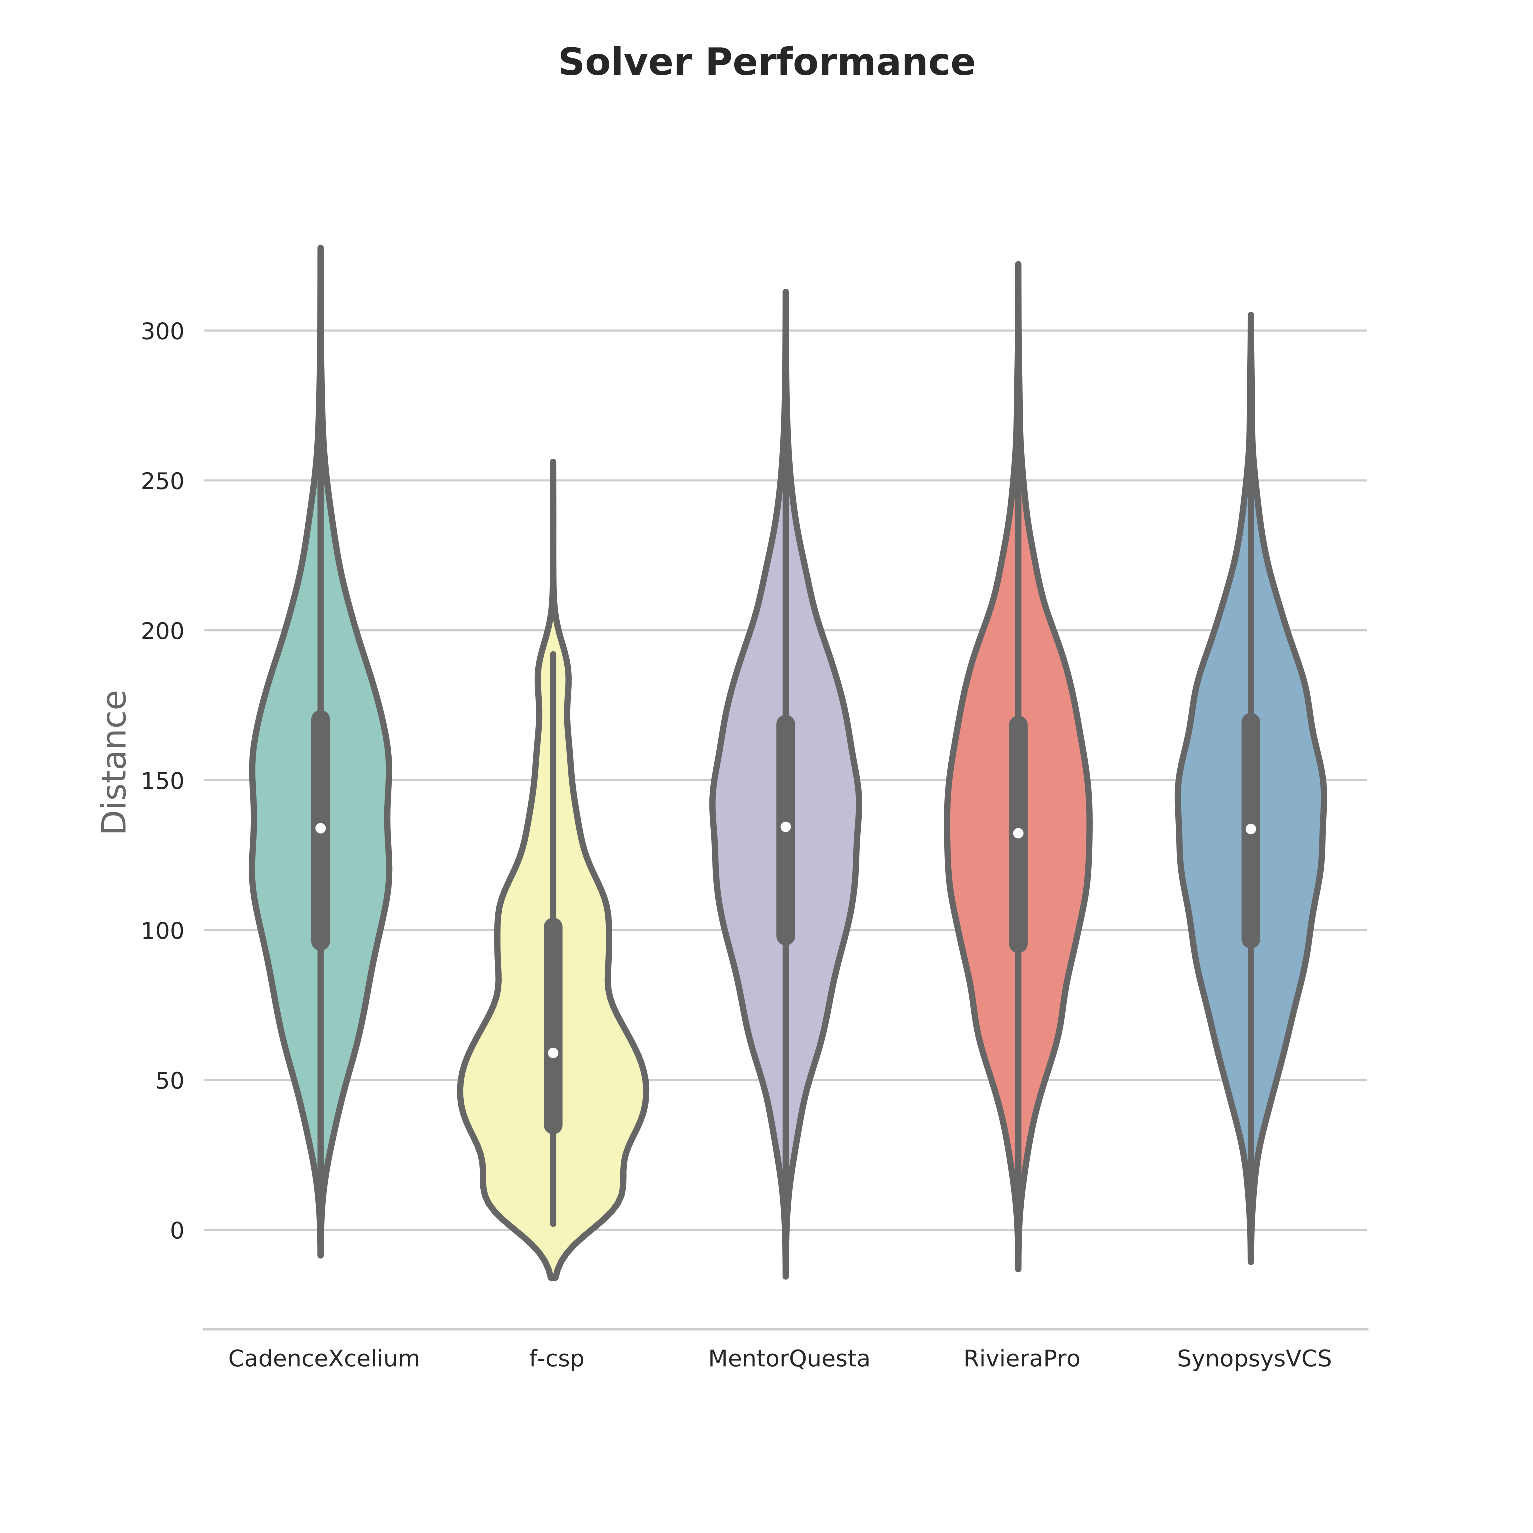
\includegraphics[width=0.7\linewidth]{pictures/F-CSP_performances.eps}
\caption{F-CSP comparison with proprietary simulators.}
\label{fig:fcsp:comparison}
\end{figure}

